\documentclass[11pt,a4paper]{report}

\usepackage{graphicx}
\usepackage{titlesec}
\usepackage{tocloft}
\usepackage{acro}
\usepackage{multirow}
\usepackage[table]{xcolor}
\usepackage{array}
\usepackage{tabularx}
\usepackage{longtable}
\usepackage{float}
\usepackage{setspace}
\usepackage{booktabs}
\usepackage{enumitem}
\usepackage{tikz}
\usetikzlibrary{arrows.meta,positioning,shapes.geometric}

\usepackage[numbers,sort&compress]{natbib}
\usepackage[breaklinks]{hyperref}
\usepackage[left=1in,right=1in,top=1in,bottom=1in]{geometry}

\renewcommand{\cfttoctitlefont}{\hfill\Large\bfseries}
\renewcommand{\cftaftertoctitle}{\hfill}
\renewcommand{\cftloftitlefont}{\hfill\Large\bfseries}
\renewcommand{\cftafterloftitle}{\hfill}
\renewcommand{\cftlottitlefont}{\hfill\Large\bfseries}
\renewcommand{\cftafterlottitle}{\hfill}

\DeclareAcronym{FM}{
  short = FM,
  long  = Facility Management
}
\DeclareAcronym{CMMS}{
  short = CMMS,
  long  = Computerized Maintenance Management System
}
\DeclareAcronym{BIM}{
  short = BIM,
  long  = Building Information Modelling
}
\DeclareAcronym{NLP}{
  short = NLP,
  long  = Natural Language Processing
}
\DeclareAcronym{ML}{
  short = ML,
  long  = Machine Learning
}
\DeclareAcronym{LSTM}{
  short = LSTM,
  long  = Long Short-Term Memory
}
\DeclareAcronym{SLA}{
  short = SLA,
  long  = Service Level Agreement
}
\DeclareAcronym{UoR}{
  short = UoR,
  long  = University of Ruhuna
}

\begin{document}

\hypersetup{pageanchor=false}
\thispagestyle{empty}

\begin{center}


\includegraphics[width=2cm,keepaspectratio=true]{uor_logo.jpg}

\vspace{1.5cm}
\begin{huge}
AI-Assisted University Maintenance Work Order Management System
\end{huge}\\
\vspace{1cm}

\begin{normalsize}
An undergraduate project proposal report submitted to the
\end{normalsize}\\
\vspace{1cm}

\begin{large}
Department of Electrical and Information Engineering\\
Faculty of Engineering\\
University of Ruhuna\\
Sri Lanka
\end{large}\\

\vspace{1cm}

\begin{normalsize}
in partial fulfillment of the requirements for the
\end{normalsize}\\
\vspace{1cm}

\begin{large}
\textbf{Degree of the Bachelor of the Science of Engineering Honours}
\end{large}\\

\vspace{1cm}
\begin{normalsize}
by
\end{normalsize}
\vspace{1cm}

\begin{tabular}[h]{lll}
Ashfaq M.R.M. & - & EG/2021/4417\\
Jathurshan T & - & EG/2021/4568
\end{tabular}\\
\vspace{1cm}

10th of April 2026\\
\vspace{1cm}

.............................................. \\
Dr. Iromi Ranaweera
\\
(Supervisor)

\end{center}

\clearpage
\hypersetup{pageanchor=true}

\pagenumbering{roman}
\setstretch{1.0}

\chapter*{Abstract}
University maintenance units handle a wide range of corrective requests for classrooms, laboratories, offices, hostels, toilets, and common spaces. In many Sri Lankan universities, including the University of Ruhuna, request handling still depends heavily on manual reading, prioritization, assignment, and follow-up. This creates delays, inconsistent priority decisions, uneven staff utilization, and weak visibility into the maintenance backlog. The problem becomes more severe when large numbers of requests arrive at the same time and when decisions rely on the experience of a small number of officers rather than on historical evidence.

This proposal presents an \ac{ML}-enabled decision-support system titled \textit{AI-Assisted University Maintenance Work Order Management System}. The proposed system uses historical maintenance work orders to support five linked functions: request intake and text preprocessing, issue classification, priority prediction, staff or trade recommendation, and schedule recommendation with final officer review. The solution is intentionally scoped as a human-in-the-loop platform rather than a fully autonomous dispatcher so that operational control remains with the university maintenance office.

The methodology combines text preprocessing, baseline classification models such as TF-IDF with Logistic Regression or Support Vector Machines, and sequence-learning models such as \ac{LSTM} or Bi-LSTM for comparison. For scheduling, the project proposes a rule-based heuristic that considers predicted priority, estimated task duration, trade availability, and workload balance. Evaluation will be based on anonymized historical records and simulated future workloads, using metrics such as classification accuracy, macro-F1, top-1 team recommendation accuracy, average response delay, overdue work orders, and workload balance.

The expected contribution is a practical engineering framework that helps the university process maintenance requests more consistently and efficiently than current manual practice.
\newpage

\tableofcontents
\newpage

\listoffigures
\newpage

\listoftables
\newpage

\addcontentsline{toc}{chapter}{Acronyms}
\acuseall
\printacronyms
\newpage

\pagenumbering{arabic}
\setcounter{secnumdepth}{3}

\chapter{Introduction}
\section{Background}
Maintenance management is a critical operational function in higher education institutions because the quality of classrooms, laboratories, offices, libraries, hostels, and public amenities directly affects teaching, research, safety, and student welfare. Although digital tools such as \ac{CMMS}, \ac{BIM}, and data repositories have become more common in \ac{FM}, many organizations still struggle to convert maintenance records into timely operational decisions \cite{matarneh2019,yang2019}. The gap is not only technological; it is also procedural. Maintenance offices often receive a large volume of requests in free-text form, after which staff must manually interpret the fault, judge urgency, identify the appropriate trade, and find a suitable slot in an already constrained work schedule.

The same challenge is visible in university settings. Educational institutions manage diverse building types and user groups, and their work-order streams contain repeated but highly varied issues such as electrical faults, plumbing leaks, air-conditioning failures, furniture damage, and sanitary problems. Historical work-order data in such environments is valuable because it captures issue patterns, response histories, team assignments, and completion times \cite{besiktepe2019}. However, unless that data is structured and analyzed, the maintenance office remains dependent on individual experience and manual triage.

Recent studies show that \ac{NLP} and predictive models can learn from maintenance request text and support classification, priority prediction, and workforce recommendation \cite{bouabdallaoui2020,mo2020,dorazio2023,ensafi2024}. These findings make a university-focused decision-support system technically feasible. For the University of Ruhuna, such a system is relevant because it can improve consistency in maintenance decisions, reduce avoidable delays, and help maintenance officers respond more effectively under limited staffing and budget conditions.

\section{Problem Statement}
The current manual approach to handling university maintenance work orders is slow, inconsistent, and difficult to scale. Free-text requests must be interpreted manually, priority is often assigned using subjective judgment, the appropriate trade team is selected based on staff experience, and scheduling decisions are made with limited visibility into workload and urgency. As a result, the university may experience delayed response to urgent issues, inconsistent handling of similar requests, poor staff utilization, and weak monitoring of backlog and overdue tasks.

This research addresses the problem of how to design a data-driven maintenance work-order management system that uses historical requests to classify issues, predict priority, recommend the most suitable maintenance team, and suggest a practical schedule more efficiently than current manual practice while keeping final approval with the maintenance officer.

\section{Objectives and Scope}
\subsection{Objectives}
The main objective of this research is to design a practical decision-support system for university corrective maintenance operations using historical work-order records.

The specific objectives are as follows:
\begin{enumerate}[label=\arabic*.]
    \item Build a historical-data-driven framework for processing maintenance work orders in a university setting.
    \item Classify maintenance request type from free-text descriptions submitted by end users.
    \item Predict the priority level of each request to support more consistent triage.
    \item Recommend the most suitable maintenance team or trade for each request.
    \item Generate a schedule recommendation under limited staff availability and officer constraints.
    \item Evaluate whether the proposed system improves response quality relative to manual practice using historical and simulated workloads.
\end{enumerate}

\subsection{Scope and Limitations}
The proposed work is intentionally bounded to remain technically sound and feasible as an academic project.
\begin{itemize}[leftmargin=1.5em]
    \item The project focuses on \textbf{corrective maintenance} requests rather than major renovation or capital works.
    \item The domain is limited to \textbf{routine university buildings and services}, such as classrooms, laboratories, offices, hostels, and common facilities.
    \item The proposed system is a \textbf{decision-support tool}; it does not fully automate field execution or remove human approval.
    \item The proposal assumes access to \textbf{anonymized historical work-order data}, but it does not claim that a live campus deployment has already been secured.
    \item Evaluation will rely on \textbf{historical records and simulated future workloads} rather than a production rollout.
    \item Preventive maintenance, spare-parts procurement, and contractor tender management are outside the current scope.
\end{itemize}

The project is significant because it targets a real university service problem and proposes an engineering solution that is both practical and evidence-driven. By reducing dependence on tacit knowledge alone, the system can support faster and more consistent maintenance decisions in a resource-constrained institutional setting.

\chapter{Literature Review}
\section{Digitization of Facility Maintenance and Current Limitations}
\ac{FM} has gradually adopted digital systems such as \ac{CMMS}, \ac{BIM}, and analytics platforms to improve data access and workflow visibility \cite{matarneh2019,yang2019}. Even so, digital adoption does not automatically solve day-to-day maintenance decision making. Bouabdallaoui et al. observed that maintenance request handling in buildings often remains manual and time-consuming despite the use of digital platforms \cite{bouabdallaoui2020}. In practice, requests arrive as unstructured text, essential fields may be missing, and officers must still interpret urgency and assign responsibility manually.

Work-order data can provide operational insight when treated as an asset instead of a passive archive. Besiktepe et al. analyzed maintenance records from educational institutions and showed that historical work-order data can reveal recurring issue patterns and support better maintenance planning \cite{besiktepe2019}. Similarly, Besiktepe et al. later highlighted that maintenance decisions depend on multiple criteria rather than on a single urgency label, reinforcing the need for structured decision support \cite{besiktepe2020}.

\section{NLP for Maintenance Request Classification}
The free-text nature of maintenance requests makes \ac{NLP} a natural starting point for automation. Bouabdallaoui et al. proposed an \ac{NLP}-based model for classifying maintenance requests in buildings and reported that text-mining methods are effective for handling unstructured maintenance descriptions \cite{bouabdallaoui2020}. Their work is important because it demonstrates that the wording of user requests contains enough signal to support early-stage routing and categorization.

For the present proposal, this literature suggests that text preprocessing, tokenization, normalization, and vectorization should be treated as a core design step rather than as a minor implementation detail. It also implies that the system must be designed for imperfect, user-generated text rather than for carefully curated technical records.

\section{Machine Learning for Priority Prediction}
Beyond classification, maintenance offices must decide how urgent a request is. Ensafi et al. reported that current prioritization practices are often user-driven and inconsistent, creating delays and decision variability \cite{ensafi2024}. Their study demonstrates the value of neural-network-based prioritization for building operations and supports the idea that historical work-order data can be used to standardize future triage.

D'Orazio et al. further showed that recurrent neural networks such as \ac{LSTM} and Bi-LSTM can predict both priority and the required technical staff from maintenance request text with high accuracy in a corrective maintenance setting \cite{dorazio2023}. This is directly relevant to the proposed university system because it confirms that sequence-based models can capture semantic patterns that simpler rules may miss.

\section{Automated Staff Assignment and Scheduling Support}
Mo et al. addressed automated staff assignment for building maintenance using \ac{NLP} and campus-scale maintenance data, showing that the same request text used for classification can also inform workforce selection and priority prediction \cite{mo2020}. This is especially relevant for universities where the wrong first assignment causes delays, repeat dispatching, and unnecessary backlog growth.

Scheduling remains a distinct challenge because assignment alone does not guarantee timely completion. Chen et al. proposed a \ac{BIM}-based framework for automatically scheduling maintenance work orders, demonstrating that scheduling quality depends on combining task information with resource and time constraints \cite{chen2018}. Beauregard and Ayer likewise emphasized the role of decision-support tools in institutional facility maintenance \cite{beauregard2019}. Lavy et al. showed that better-structured information can improve work-order processing time \cite{lavy2019}. Taken together, these studies suggest that a realistic university solution should not stop at classifying requests; it must link prediction outputs to a usable scheduling recommendation.

\section{Research Gap}
The literature shows clear progress in four separate areas: digitization of \ac{FM} data, text-based request classification, priority prediction, and team assignment. However, three important gaps remain.

First, many studies address only one step in the work-order pipeline, while university maintenance operations require an integrated chain from \textit{classify} to \textit{prioritize} to \textit{assign} to \textit{schedule}. Second, several works are based on hospitals or generic building portfolios, whereas the educational-campus context has its own mix of assets, users, and service expectations \cite{besiktepe2019}. Third, many intelligent approaches are presented as prediction models, but operational improvement also depends on how model outputs are translated into human-reviewable schedules under staffing constraints.

Therefore, the proposed research fills a practical gap by designing a university-focused, human-in-the-loop decision-support framework that integrates classification, priority prediction, team recommendation, and schedule recommendation in a single workflow.

\section{Summary of Literature}
\begin{table}[H]
\centering
\small
\caption{Summary of prior work and the gap addressed by the proposed project}
\begin{tabularx}{\textwidth}{|p{3cm}|X|X|}
\hline
\textbf{Study focus} & \textbf{Main contribution} & \textbf{Limitation relative to this project} \\
\hline
Maintenance request classification \cite{bouabdallaoui2020} & Demonstrates that \ac{NLP} can classify unstructured maintenance request text. & Does not integrate prioritization, team recommendation, and scheduling into one decision flow. \\
\hline
Staff assignment from request text \cite{mo2020} & Predicts workforce and priority from campus maintenance data. & Focuses on prediction accuracy more than end-to-end scheduling and officer review workflow. \\
\hline
Priority and technical staff prediction \cite{dorazio2023} & Shows strong performance of \ac{LSTM}/Bi-LSTM for priority and staff prediction. & Case setting is not tailored to Sri Lankan university operations and does not provide a full scheduling layer. \\
\hline
Work-order prioritization using neural networks \cite{ensafi2024} & Highlights inconsistency in manual prioritization and validates a data-driven alternative. & Concentrates on prioritization and data preparation rather than integrated assignment and scheduling. \\
\hline
Educational maintenance data analysis \cite{besiktepe2019} & Shows the value of historical work-order data in educational institutions. & Exploratory in nature and does not propose a complete predictive decision-support pipeline. \\
\hline
Automatic maintenance scheduling \cite{chen2018} & Connects task information to automated work-order scheduling. & Requires integration with classification and priority models for practical triage of text-based requests. \\
\hline
\end{tabularx}
\end{table}

\chapter{Research Methodology}
\section{Research Design}
This project follows a design-and-evaluate methodology. The research begins with requirement analysis and literature study, followed by preparation of anonymized historical work-order data. The system is then developed as a linked set of predictive and rule-based modules. Finally, its performance is evaluated on historical and simulated workloads against metrics relevant to the university maintenance office.

The proposed system is designed as a human-in-the-loop workflow. Model outputs are recommendations, not automatic final decisions. The maintenance officer remains responsible for approval, exception handling, and operational override.

\section{Proposed System Architecture}
\begin{figure}[H]
\centering
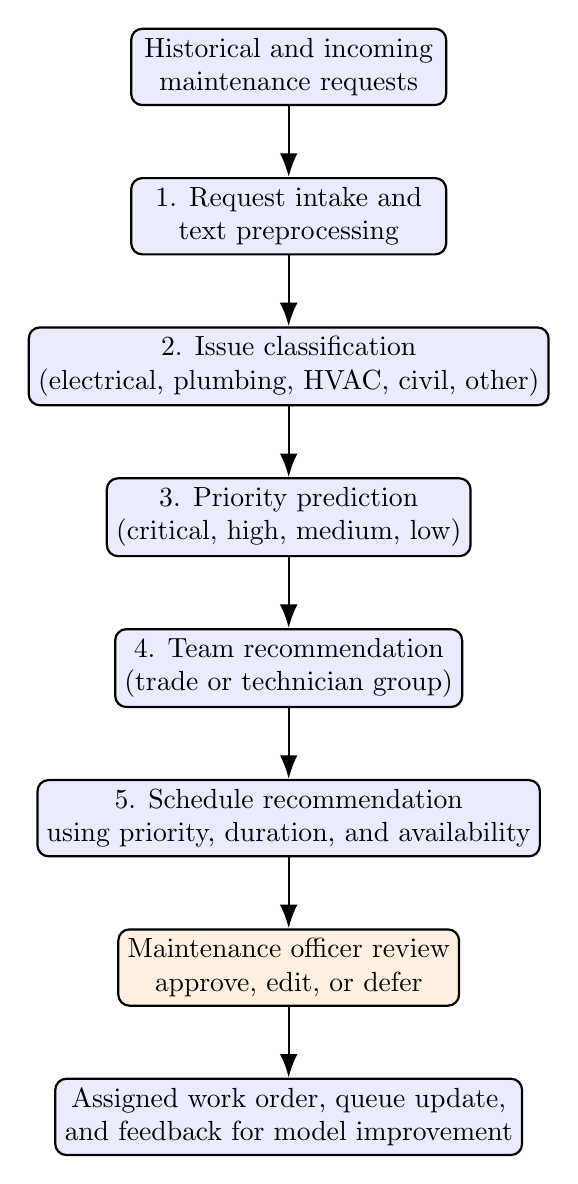
\begin{tikzpicture}[
    node distance=0.9cm and 0.6cm,
    block/.style={rectangle, rounded corners, draw=black, thick, align=center, minimum width=4cm, minimum height=0.95cm, fill=blue!8},
    decision/.style={rectangle, rounded corners, draw=black, thick, align=center, minimum width=4cm, minimum height=0.95cm, fill=orange!12},
    arrow/.style={-{Latex[length=3mm]}, thick}
]
\node[block] (input) {Historical and incoming\\maintenance requests};
\node[block, below=of input] (pre) {1. Request intake and\\text preprocessing};
\node[block, below=of pre] (classify) {2. Issue classification\\(electrical, plumbing, HVAC, civil, other)};
\node[block, below=of classify] (priority) {3. Priority prediction\\(critical, high, medium, low)};
\node[block, below=of priority] (team) {4. Team recommendation\\(trade or technician group)};
\node[block, below=of team] (schedule) {5. Schedule recommendation\\using priority, duration, and availability};
\node[decision, below=of schedule] (review) {Maintenance officer review\\approve, edit, or defer};
\node[block, below=of review] (output) {Assigned work order, queue update,\\and feedback for model improvement};

\draw[arrow] (input) -- (pre);
\draw[arrow] (pre) -- (classify);
\draw[arrow] (classify) -- (priority);
\draw[arrow] (priority) -- (team);
\draw[arrow] (team) -- (schedule);
\draw[arrow] (schedule) -- (review);
\draw[arrow] (review) -- (output);
\end{tikzpicture}
\caption{Workflow of the proposed university maintenance decision-support system}
\label{fig:architecture}
\end{figure}

Figure \ref{fig:architecture} illustrates the intended workflow. Incoming requests and historical records enter the preprocessing stage, where text and metadata are cleaned and standardized. The issue category is predicted first because it supports the downstream choice of trade team. Priority prediction then determines operational urgency. The staff recommendation module uses both the request content and the predicted category and priority to identify the most suitable team. Finally, a schedule recommendation is generated and presented to the maintenance officer for approval.

\section{Historical Data Schema}
The project assumes access to anonymized historical maintenance records with the schema shown in Table \ref{tab:schema}. The attributes are sufficient for both predictive modeling and scheduling analysis.

\begin{table}[H]
\centering
\caption{Assumed historical work-order data schema}
\label{tab:schema}
\begin{tabularx}{\textwidth}{|p{3.2cm}|p{2.5cm}|X|}
\hline
\textbf{Field} & \textbf{Type} & \textbf{Purpose} \\
\hline
\texttt{request\_id} & Identifier & Unique reference for each maintenance work order. \\
\hline
\texttt{submitted\_date\_time} & Date/time & Supports trend analysis, backlog analysis, and scheduling logic. \\
\hline
\texttt{building/location} & Categorical & Indicates where the issue occurred and supports workload balancing by location. \\
\hline
\texttt{request\_text} & Free text & Main input for classification, priority prediction, and team recommendation. \\
\hline
\texttt{issue\_category} & Label & Historical target label for request-type classification. \\
\hline
\texttt{priority\_level} & Label & Historical target label for urgency prediction. \\
\hline
\texttt{assigned\_team/trade} & Label & Historical target label for team recommendation. \\
\hline
\texttt{completion\_time} & Numeric/time & Supports service-duration estimation and schedule quality analysis. \\
\hline
\texttt{status} & Categorical & Indicates whether the request is open, in progress, completed, or overdue. \\
\hline
\end{tabularx}
\end{table}

\section{Module-Level Methodology}
\subsection{Module 1: Request Intake and Text Preprocessing}
The preprocessing stage converts free-text requests into a structured representation suitable for prediction. This stage includes text normalization, lowercasing, punctuation handling, tokenization, spelling cleanup where feasible, stop-word handling, and conversion into numerical features such as TF-IDF vectors. Historical metadata such as location and submission time may be encoded as supporting features when useful.

\subsection{Module 2: Issue Classification}
The second module predicts the maintenance issue category from the request text. Baseline models such as TF-IDF with Logistic Regression or Support Vector Machines will be used first because they are interpretable and computationally efficient. Their results will form a benchmark against which sequence models can be compared.

\subsection{Module 3: Priority Prediction}
The priority module predicts whether a request should be treated as critical, high, medium, or low priority. The problem will be approached as supervised multi-class classification. In addition to baseline text models, recurrent architectures such as \ac{LSTM} and Bi-LSTM will be tested because previous maintenance studies have shown that they can capture ordering and context in request text effectively \cite{dorazio2023}.

\subsection{Module 4: Staff or Team Recommendation}
This module predicts the most suitable trade team, such as electrical, plumbing, civil, HVAC, or general maintenance. The intent is not to replace the maintenance office but to reduce first-assignment errors. The model will use the request text together with predicted category and priority signals to recommend the most relevant team. Performance will be assessed using top-1 accuracy and confusion patterns between related trades.

\subsection{Module 5: Schedule Recommendation with Officer Review}
The scheduling component will use a rule-based heuristic rather than a fully autonomous optimizer. Each new request will be ranked using predicted priority, expected duration, location, team availability, and current workload. The output will be a recommended service slot or queue position that the maintenance officer can approve, adjust, or defer. This design is appropriate because it aligns with real operational practice while remaining implementable within the project scope.

\section{System Inputs, Outputs, and Evaluation}
The principal system inputs are historical maintenance records and new incoming requests. The key outputs are:
\begin{itemize}[leftmargin=1.5em]
    \item predicted issue category,
    \item predicted priority level,
    \item recommended maintenance team or trade,
    \item suggested schedule position or time slot,
    \item review-ready work-order summary for the maintenance officer.
\end{itemize}

Evaluation will use train-test separation on historical records together with simulated future workloads to stress the scheduling logic. The following performance measures will be reported:
\begin{itemize}[leftmargin=1.5em]
    \item classification accuracy and macro-F1 for issue classification,
    \item accuracy and F1 for priority prediction,
    \item top-1 accuracy for team recommendation,
    \item average response delay,
    \item number of overdue work orders,
    \item workload balance across teams.
\end{itemize}

The proposed system will be considered successful if it demonstrates more consistent triage and assignment decisions than current manual practice while remaining transparent enough for officer review and operational adoption.

\section{Expected Resources and Implementation Tools}
The prototype can be implemented using open-source software. Python will be used for data preparation and modeling, with libraries such as Pandas, Scikit-learn, and either TensorFlow or PyTorch. A lightweight database or spreadsheet export can store cleaned work-order data. A simple prototype interface may be developed for demonstration, but the emphasis of the proposal is on the decision-support pipeline rather than on a production web platform.

\section{Time Plan and Budget}
\subsection{Time Plan}
\renewcommand{\arraystretch}{1.25}
\setlength{\tabcolsep}{5pt}

\begin{table}[H]
\centering
\caption{Proposed project time plan from May 2026 to October 2026}
\begin{tabular}{|p{6.2cm}|c|c|c|c|c|c|}
\hline
\textbf{Activity} & \textbf{May} & \textbf{Jun} & \textbf{Jul} & \textbf{Aug} & \textbf{Sep} & \textbf{Oct} \\
\hline
Requirement study and literature review & \cellcolor{blue!20} & \cellcolor{blue!20} &  &  &  &  \\
\hline
Data collection, cleaning, and anonymization &  & \cellcolor{blue!20} & \cellcolor{blue!20} &  &  &  \\
\hline
Feature engineering and baseline models &  &  & \cellcolor{green!20} & \cellcolor{green!20} &  &  \\
\hline
Bi-LSTM model development and comparison &  &  &  & \cellcolor{green!20} & \cellcolor{green!20} &  \\
\hline
Staff recommendation and scheduling logic &  &  &  & \cellcolor{yellow!30} & \cellcolor{yellow!30} &  \\
\hline
Prototype interface and module integration &  &  &  &  & \cellcolor{orange!30} & \cellcolor{orange!30} \\
\hline
Evaluation, analysis, and report writing &  &  &  &  & \cellcolor{red!20} & \cellcolor{red!20} \\
\hline
\end{tabular}
\end{table}


\subsection{Estimated Budget}
Table \ref{tab:budget} presents the estimated budget for developing a prototype-level system. Since the work is a proposal-stage academic project, open-source software is assumed wherever possible.

\begin{table}[H]
\centering
\caption{Estimated prototype budget}
\label{tab:budget}
\begin{tabular}{|p{8cm}|r|}
\hline
\textbf{Item} & \textbf{Estimated Cost (LKR)} \\
\hline
Software tools and libraries (open source) & 0 \\
\hline
Cloud, internet, and compute allowance & 20,000 \\
\hline
Data preparation and annotation allowance & 15,000 \\
\hline
Prototype server or workstation contribution & 35,000 \\
\hline
Meetings, transport, and printing & 10,000 \\
\hline
Contingency & 8,000 \\
\hline
\textbf{Total} & \textbf{88,000} \\
\hline
\end{tabular}
\end{table}

\subsection{Resource Justification}
The proposed budget is modest because the project emphasizes data-driven decision support rather than large hardware procurement. The main cost drivers are computing access, data preparation effort, and basic project logistics. Open-source \ac{ML} libraries keep software cost at zero, which is suitable for a university prototype.

\section{Conclusion}
This proposal addresses a practical and community-relevant problem: the inefficient handling of university maintenance work orders under manual practice. The proposed \textit{AI-Assisted University Maintenance Work Order Management System} uses historical maintenance requests to support issue classification, priority prediction, staff recommendation, and schedule recommendation while keeping the maintenance officer in control of the final decision.

The project is feasible because it builds on methods already validated in the maintenance and \ac{FM} literature, especially \ac{NLP}-based classification, neural-network-based prioritization, and predictive team assignment \cite{bouabdallaoui2020,mo2020,dorazio2023,ensafi2024}. Its contribution is to integrate these ideas into a single university-focused workflow that is realistic for Sri Lankan institutional settings. If implemented, the system can improve consistency, reduce avoidable delays, and provide a stronger evidence base for maintenance planning at the University of Ruhuna.

\renewcommand{\bibname}{References}
\bibliographystyle{ieeetr}
\addcontentsline{toc}{chapter}{References}
\bibliography{bibliography}

\end{document}
